%%%%%%%%%%%%%%%%%%%%%%%%%%%%%%%%%%%%%%%%%%%%%%%%%%%
%% LaTeX book template                           %%
%% Author:  Amber Jain (http://amberj.devio.us/) %%
%% License: ISC license                          %%
%%%%%%%%%%%%%%%%%%%%%%%%%%%%%%%%%%%%%%%%%%%%%%%%%%%

\documentclass[a4paper,11pt,oneside]{book}

% pacotes utilizados
\usepackage[T1]{fontenc}
\usepackage[utf8]{inputenc}
\usepackage{lmodern}
\usepackage{hyperref}
\usepackage{graphicx}
\usepackage[portuguese]{babel}
\usepackage{amsfonts}
\usepackage[usenames,dvipsnames]{xcolor}
\usepackage{mathtools}
\usepackage{amssymb} % alguns simbolos matematicos
\usepackage{mathrsfs} % letras cursivas
\usepackage{listings} % coding examples in latex file
\usepackage{xcolor} % changing colors
\usepackage{amsthm} % definir estilo do teorema
\usepackage[hang,flushmargin]{footmisc} % remove footnote's identation
\usepackage{cancel} % para poder colocar o tracinho de cancelamento
\usepackage{tikz} % to draw Venn's diagrams
\usepackage{amsmath} % to write a function by cases
\usepackage{graphicx} % to set a images directory
\usepackage{caption} % to supress numbering in figures
\usepackage{float} % to make a figure stay when i whant

\graphicspath{{./images/}} % set an default images folder

% dark theme no pdf
\pagecolor[rgb]{0.1,0.1,0.1} %black
\color[rgb]{0.9,0.9,0.9} %grey

% criando o modelo de definicoes/teoremas/fatos/demonstracoes
\theoremstyle{definition}

\newtheoremstyle{break}% name
  {10pt}%         Space above, empty = `usual value'
  {10pt}%         Space below
  {}% Body font
  {}%         Indent amount (empty = no indent, \parindent = para indent)
  {\bfseries}% Thm head font
  {}%        Punctuation after thm head
  {\newline}% Space after thm head: \newline = linebreak
  {}%         Thm head spec

\theoremstyle{break}

% definindo as categorias de formalidade
\newtheorem{definition}{Definição}[section]
\newtheorem{fact}{Fato}[section]
\newtheorem{demonstration}{Demonstração}[section]
\newtheorem{theorem}{Teorema}

% tirando identação dos paragrafos
\setlength{\parindent}{0ex}

% setting das cores quando usar codigo python
\definecolor{codegreen}{rgb}{0,0.6,0}
\definecolor{codegray}{rgb}{0.5,0.5,0.5}
\definecolor{codepurple}{rgb}{0.58,0,0.82}
\definecolor{backcolour}{rgb}{0.95,0.95,0.92}

\lstdefinestyle{mystyle}{
    backgroundcolor=\color{backcolour},   
    commentstyle=\color{codegreen},
    keywordstyle=\color{magenta},
    numberstyle=\tiny\color{codegray},
    stringstyle=\color{codepurple},
    basicstyle=\ttfamily\footnotesize,
    breakatwhitespace=false,         
    breaklines=true,                 
    captionpos=b,                    
    keepspaces=true,                 
    numbers=left,                    
    numbersep=5pt,                  
    showspaces=false,                
    showstringspaces=false,
    showtabs=false,                  
    tabsize=2
}

\lstset{style=mystyle}

% dedicatoria 
% Source: http://www.tug.org/pipermail/texhax/2010-June/
\newenvironment{dedication}
{
   \cleardoublepage
   \thispagestyle{empty}
   \vspace*{\stretch{1}}
   \hfill\begin{minipage}[t]{0.66\textwidth}
   \raggedright
}
{
   \end{minipage}
   \vspace*{\stretch{3}}
   \clearpage
}

% Chapter quote at the start of chapter        %
% Source: http://tex.stackexchange.com/a/53380 %
\makeatletter
\renewcommand{\@chapapp}{}% Not necessary...
\newenvironment{chapquote}[2][2em]
  {\setlength{\@tempdima}{#1}%
   \def\chapquote@author{#2}%
   \parshape 1 \@tempdima \dimexpr\textwidth-2\@tempdima\relax%
   \itshape}
  {\par\normalfont\hfill--\ \chapquote@author\hspace*{\@tempdima}\par\bigskip}
\makeatother


%%%%%%%%%%%%%%%%%%%%%%%%%%%%%%%%%%%%%%%%%%%%%%%%%%%
% First page of book which contains 'stuff' like: %
%  - Book title, subtitle                         %
%  - Book author name                             %
%%%%%%%%%%%%%%%%%%%%%%%%%%%%%%%%%%%%%%%%%%%%%%%%%%%
% Book's title and subtitle
\title{\Huge \textbf{Microeconomia} \\ 
\Large Tradução da 9 edição \\
\huge Hal R. Varian}

% Author
\author{
\textsc{Resumo e Adaptação por:} \\
\textsc{Bruno de M. Ruas}
}

\begin{document}

\frontmatter
\maketitle

\tableofcontents
%\listoffigures
%\listoftables

\mainmatter

%%%%%%%%%%%%%%%%%%%%%%%% PART %%%%%%%%%%%%%%%%%%%%%%%%
\part*{Preparativos}
\addcontentsline{toc}{part}{Preparativos}

%%%%%%%%%%%%%%%%%%%%%%%% CHAPTER %%%%%%%%%%%%%%%%%%%%%%%%
\chapter*{Matemática}
\addcontentsline{toc}{chapter}{Matemática}

\begin{chapquote}{The Godfather}
	``Some Day, And That Day May Never Come, I Will Call Upon You To Do A Service For Me.''.
\end{chapquote}

Bem vindo ao meu resumo do livro do prof. Varian. Ao contrário do que ele fez, eu preferi trazer o apêndice de matemática pro começo do material porque aqui nós vamos ver as ferramentas que serão usadas para a explicação dos conceitos teóricos ao longo do material.
\\
\\
Aqui a gente só vai dar um overview básico nos conceitos. Não tenha dúvida que alguém mais experimentado em matemática torceria o nariz pra algumas definições dadas aqui. Mas o objetivo é te dar um "norte"\ a respeito de alguns conceitos normalmente usados. Não se assuste com a simplicidade de algumas coisas. Melhor garantir agora do que sofrer mais pra frente no texto.

\section*{Funções}
\addcontentsline{toc}{section}{Funções}

Sejam dois números quaisquer $x$ e $y$, uma \textbf{função} ou \textbf{transformação} é uma regra que descreve uma relação entre eles.
\\
\\
Para demonstrar que existe alguma dependência entre duas variáveis usamos a notação $y = f(x)$, onde nossa variável $y$ (chamada de \textbf{dependente}) é o resultado de alguma transformação (denotada pelo símbolo $"f"$) realizada em $x$ (nossa variável \textbf{independente}).
\\
\\
Não é raro ter uma variável dependente relacionada a várias outras variáveis. Nesses casos é comum o uso da notação anterior com a adição das novas incógnitas. Algo como $y = f(x_1,x_2,...,x_n)$.

\section*{Gráficos}
\addcontentsline{toc}{section}{Gráficos}

Não tem muito o que falar aqui. Dá uma lida lá na página 1010.

\section*{Propriedades das Funções}
\addcontentsline{toc}{section}{Propriedades das Funções}

Uma função pode ter algumas características que facilitam a sua descrição. Aqui temos algumas que serão usadas ao longo do curso:
\\
\\
Uma \textbf{função contínua} é aquela que não possui nenhum "salto"\ ou "quebra". 
\\
\\
Uma \textbf{função suave} é aquela que não tem "dobras"\ nem "cantos".
\\
\\
Uma \textbf{função monotônica} é aquela que sempre segue o mesmo sentido (ou crescendo ou decrescendo) sem nunca mudar de sentido. 
Quando é crescente a medida que $x$ cresce, chamaremos de \textbf{função monotônica crescente}. Quando decrescer a medida que $x$ crescer, chamaremos de \textbf{função monotônica decrescente}.

\section*{Funções Inversas}
\addcontentsline{toc}{section}{Funções Inversas}

Uma das implicações de quando uma função é monotônica é que, para cada $x$, sempre existirá apenas um único $y$ associado. 
\\
\\
Uma \textbf{função inversa} é a função que, sempre que colocarmos um $y$ como variável independente teremos como resultado um $x$ de alguma função anterior.\footnote{Eu tentei não deixar confuso mas se ficou com dúvida, pesquisa um pouco sobre o tema.}

\section*{Equações e Identidades}
\addcontentsline{toc}{section}{Equações e Identidades}

Podemos relacionar dois ou mais elementos por meio do uso de \textbf{equações} (usando o símbolo da igualdade "$=$"). Onde as suas respectivas \textbf{soluções} são os valores atribuíveis as incógnitas que assegurem a validade da relação proposta.
\\
\\
Uma \textbf{identidade} (que tem o símbolo dado por "$\equiv$") é um tipo de relação onde sempre haverá as soluções independentemente de quais valores suas variáveis assumam.

\section*{Funções Lineares}
\addcontentsline{toc}{section}{Funções Lineares}

Chamamos de \textbf{função linear}, qualquer função da forma $y = ax + b$. Fique atento porque uma função linear pode ser expressa de maneira implícita (ou seja, será necessário desenvolver um pouco a álgebra até que se chegue numa equação no formato da definição).

\section*{Variações e Taxas de Variação}
\addcontentsline{toc}{section}{Variações e Taxas de Variação}

Usamos o símbolo "$\Delta$"\footnote{O nome é "delta".} para denotar a variação de alguma variável. Ou seja, se tivemos uma variável qualquer $x$ que teve seu valor alterado de $x^1$ para $x^2$, então:

$$ \Delta x = x^2 - x^1 $$
ou também
$$ x^2 = x^1 + \Delta x $$
\\
Normalmente, usamos o delta quando falamos de \textbf{pequenas variações} ou, como os economistas falam, \textbf{variações marginais}.
\\
\\
A \textbf{taxa de variação} é obtida pela razão (ou seja, pela divisão) de duas variações. Seja a função $y = f(x)$, sempre que tivemos um $\Delta x > 0$ também teremos algum $\Delta y \neq 0$. A taxa de variação de $y$ em relação à $x$ é dada por:

$$ \frac{\Delta y}{\Delta x} = \frac{y^2 - y^1}{x^2 - x^1} = \frac{f(x^1 + \Delta x) - f(x^1)}{\Delta x} $$
\\
É uma medida do quanto $y$ varia a medida que $x$ varia.
\\
\\
Quando uma função é linear, teremos que essa taxa de variação será sempre constante para quaisquer valores de $x$. Como $y = ax + b$, então
\\
\\
\Large $ \frac{\Delta y}{\Delta x} = $ \normalsize
$$ \frac{a+b(x^1 + \Delta x) - (a + bx^1)}{\Delta x} = $$
$$ \frac{\cancel{a}+b(x^1 + \Delta x) \cancel{-a} - bx^1)}{\Delta x} = $$
$$ \frac{\cancel{bx^1} + b \Delta x \cancel{- bx^1}}{\Delta x} = $$
$$ \frac{b \cancel{\Delta x}}{\cancel{\Delta x}} = b  $$

Para as funções não lineares, essa propriedade não é observada. Tomemos $y = f(x) = x^2$ como exemplo,
\\
\\
\Large $ \frac{\Delta y}{\Delta x} = $ \normalsize
$$ \frac{(x + \Delta x)^2 - x^2}{\Delta x} = $$ 
$$  \frac{\cancel{x^2} + 2x \Delta x + (\Delta x)^2 \cancel{-x^2}}{\Delta x} = $$
$$  \frac{2x \cancel{\Delta x} + \Delta x . \cancel{\Delta x}}{\cancel{\Delta x}} = $$
$$  2x + \Delta x $$
\\
Ou seja, entra no resultado da taxa de variação o valor de $x$ e a magnitude da variação, dada por $\Delta x$.

\section*{Inclinações e Interceptos}
\addcontentsline{toc}{section}{Inclinações e Interceptos}

Já aprendemos como calcular a taxa de variação de uma função. Graficamente falando, essa é a medida da inclinação da curva da função entre os dois pontos que formam o delta da variável independente. 
\\
\\
Em uma função linear, a inclinação da curva sempre será a mesma independente da magnitude da variação. No caso das funções não lineares, a inclinação é dada pela \textbf{reta tangente} ao ponto da curva\footnote{Mais pra frente a gente volta nessa ideia.}.
\\
\\
No caso de uma função linear, $ y = ax + b$, temos alguns pontos que recebem nomes de \textbf{intercepto}. O \textbf{intercepto vertical} ($y^*$) é dado pelo ponto $y = a.0 + b = b$, ou seja, onde $x = 0$. Já o \textbf{intercepto horizontal} ($x^*$) é dado pelo ponto onde $y = ax + b = 0 $, ou seja, $ x = \frac{-b}{a}$.

\section*{Valores absolutos e logaritmos}
\addcontentsline{toc}{section}{Valores Absolutos e Logaritmos}

O \textbf{valor absoluto} de um número $x$ qualquer é definido pela função $f(x)$ do seguinte modo:

\[ f(x) = |x| = \begin{cases} x & se \ x \geqslant \\ -x & se \ x < 0 \end{cases} \]
\\
\\
Você já deve ter visto no ensino médio que o \textbf{logaritmo natural} ou \textbf{log} de um número é uma função escrita como $y = lnx$ ou $y = ln(x)$ e que possui as seguintes propriedades:

\begin{itemize}
 \item Se $x,y > 0$, então, $ ln(xy) = ln(x) + ln(y) $
 \item $ ln(e) = 1 $
 \item $ ln(x^y) = y ln(x) $
\end{itemize}

\section*{Derivadas}
\addcontentsline{toc}{section}{Derivadas}

Você deve lembrar desse conceito das aulas de matemática no primeiro período. A \textbf{derivada} da função $f(x)$ será dada por:

$$ f'(x) = \frac{df(x)}{dx} = \lim_{\Delta x \to 0} \frac{f(x + \Delta x) - f(x)}{\Delta x} $$
\\
Mas perai, a gente acabou de ver um conceito muito parecido no ponto 1.7. E é isso mesmo, a derivada é o cálculo da taxa de variação à medida que aplicamos o limite\footnote{Vá pesquisar se você não souber o que é isso.} até $0$ para nosso $\Delta x$.
\\
\\
\textbf{Comentário}: Essa técnica é muito importante ao longo de quase todos os tópicos desse curso. Volte nas apostilas e nas listas de derivadas caso seja necessário.

\section*{Derivadas segundas}
\addcontentsline{toc}{section}{Derivadas Segundas}

Já vimos que a deriva nos permite saber a inclinação da reta tangente da nossa função genérica $f(x)$ num determinado ponto. Chamamos de \textbf{derivada segunda} de $f(x)$ a derivada da derivada dessa função.

$$ f''(x) = \frac{d^2f(x)}{dx^2} $$
\\
Nós aplicamos a derivada segunda para descobrirmos a curvatura da função no ponto $x$. Se for positiva, a função é convexa no ponto. Se for negativa, a função é côncava no ponto. Por fim, se for igual a zero, a função será plana.

\section*{A regra do produto e da cadeia}
\addcontentsline{toc}{section}{A regra do Produto e da Cadeia}

Dadas duas funções $g(x)$ e $h(x)$ Se definirmos uma nova função $f(x) = g(x) h(x)$. A derivada dessa última função é dada pela aplicação da \textbf{regra do produto}:
\\
$$ \frac{df(x)}{dx} = g(x)\frac{dh(x)}{dx} + h(x)\frac{dg(x)}{dx}$$
\\
\\
\textbf{Comentário}: Normalmente a gente vê a regra do produto e da divisão junto. Mas o prof. Varian não colocou essa segunda regra como necessária. Então se eu ver que ficou faltando, eu atualizo esse material.
\\
\\
Agora imagine a situação onde temos uma função dentro de outra função. Dadas as funções $y = g(x)$ e $z = h(y)$, a \textbf{função composta} é dada por $f(x) = h(g(x))$, cuja derivada é obtida pela seguinte regra:

$$ \frac{df(x)}{dx} = \frac{dh(y)}{dy}\frac{dg(x)}{x}$$

\section*{Derivadas parciais}
\addcontentsline{toc}{section}{Derivadas Parciais}

Nós já vimos no ponto 1.1 que funções podem conter mais de uma variável independente. Supondo uma função composta $f(x_1,x_2)$ a sua \textbf{derivada parcial} em relação a $x_1$ será dada por:

$$ \frac{\partial f(x_1,x_2)}{\partial x_1} = 
\lim_{\Delta x_1 \to 0} \frac{f(x_1+\Delta x_1,x_2) - f(x_1,x_2)}{\Delta x_1} $$
\\
similarmente, a derivada parcial em relação a $x_2$ será dada por
\\
$$ \frac{\partial f(x_1,x_2)}{\partial x_2} = 
\lim_{\Delta x_2 \to 0} \frac{f(x_1,x_2+\Delta x_2) - f(x_1,x_2)}{\Delta x_2} $$
\\
A ideia por trás de uma derivada parcial é verificar a taxa de variação entre a nossa função composta em relação a alguma variação de apenas uma das variáveis independentes, ou seja, é como se tratássemos as outras variáveis como constantes.
\\
\\
As propriedades das derivadas parciais são parecidas com as normais. Exceção é a regra da cadeia. Seja a função composta $g(t) = f(x_1(t),x_2(t))$, então a derivada de $g(t)$ em relação a $t$ é dada por:

$$ \frac{dg(t)}{dt} = 
\frac{\partial f(x_1,x_2)}{\partial x_1}\frac{dx_1(t)}{dt} + 
\frac{\partial f(x_1,x_2)}{\partial x_2}\frac{dx_2(t)}{dt} $$
\\
Atente para o fato que as variáveis independentes da nossa função $g(t)$ são as funções $x_1(t)$ e $x_2(t)$ que também têm como variável independente $t$.

\section*{Otimização}
\addcontentsline{toc}{section}{Otimização}

A maioria dos modelos utilizados pela Economia podem ser expressos como um problemas de otimização. Matematicamente falando, dada uma função $y = f(x)$ seu valor \textbf{máximo} será dado ponto $x^*$ se $f(x^*) \geqslant f(x)$ para qualquer valor de $x$. Não faz parte do escopo desse apêndice demonstrar isso, então tenha fé que, se uma função for suave, o seu valor máximo é obtido no ponto onde teremos

$$ \frac{df(x^*)}{dx} = 0 $$

e também

$$ \frac{d^2f(x^*)}{dx^2} \leq 0$$
\\
Ou seja, o máximo será o ponto onde a derivada for igual a zero e a derivada segunda for menor igual a zero. Chamamos a primeira de \textbf{condição de primeira ordem} e a segunda de \textbf{condição de segunda ordem}.
\\
\\
Também é muito comum buscarmos a minimização de determinadas funções. Nesse caso, só teremos uma pequena mudança na condição de segunda ordem;

$$ \frac{df(x^*)}{dx} = 0 $$

e também

$$ \frac{d^2f(x^*)}{dx^2} \geq 0$$
\\
No casos das funções compostas suaves, as condições de primeira ordem para os pontos de máximo e mínimo são alcançadas no ponto $(x_{1}^*,x_{2}^*)$ cujas derivadas serão

$$ \frac{\partial f(x_{1}^*,x_{2}^*)}{\partial x_1} = 0 $$
e
$$ \frac{\partial f(x_{1}^*,x_{2}^*)}{\partial x_2} = 0 $$
\\
As condições de segunda ordem são muito mais complexas então não fazem parte do escopo desse curso.

\section*{Otimização com restrição}
\addcontentsline{toc}{section}{Otimização com Restrição}

Saber maximizar ou minimizar uma função é só uma parte do problema de otimização. Na vida real, a esmagadora maioria das situações de otimização está contida dentro de algum limite de possibilidades. A \textbf{otimização com restrição} é a técnica usada para encontrar o ponto de máximo ou mínimo de alguma função dentro de um determinado domínio de possibilidades.

\begin{center}
\LARGE $\stackrel{máx}{\text{\small $x_1,x_2$}} \ \ \stackrel{f(x_1,x_2)}{\ }$ \\
\normalsize $\textrm{de modo que } g(x_1,x_2) = c$
\end{center}

A função $f(x_1,x_2)$ é chamada de \textbf{função objeto} e a equação $g(x_1,x_2) = c$ é chamada de \textbf{restrição}.

%%%%%%%%%%%%%%%%%%%%%%%% CHAPTER %%%%%%%%%%%%%%%%%%%%%%%%
\chapter*{Programação}
\addcontentsline{toc}{chapter}{Programação}

\begin{chapquote}{The Godfather}
	``I don’t like violence, Tom. I’m a businessman. Blood is a big expense.''.
\end{chapquote}


Caro aluno, com o avanço do poder computacional e da disponibilidade de dados, os economistas não ficaram de fora da revolução tecnológica. Além de todo o arcabouço teórico, matemático, estatístico, histórico e social que você está adquirindo na sua formação, a programação se tornou uma ferramenta indispensável para o processo de análise moderna e merece ser objeto do seu estudo\footnote{Pode até ser que você não tenha alguma matéria de programação na sua grade curricular, mas não se engane, mesmo que seu curso não esteja cobrando, vá estudar por conta própria.}.
\\
\\
Ao longo do livro eu vou construir alguns programas em Python para simular os modelos que a gente for construindo. Não faz parte do escopo desse livro ensinar como fazer isso. Contudo, cada código será disponibilizado em dois links. O primeiro é referente ao repositório no github e o segundo é referente a um notebook no google colab onde você pode executar o modelo sem precisar instalar nada no seu computador.

\section*{Capítulo 25 - Monopólio}
\addcontentsline{toc}{section}{Capítulo 25 - Monopólio}

\subsection*{Demanda Linear e Monopólio (25.2)}
\addcontentsline{toc}{subsection}{Demanda Linear e Monopólio (25.2)}

\begin{center}
\href{https://github.com/brunoruas2/Meus_Estudos/blob/main/Microeconomia/Microeconomics\%20-\%20Hal\%20Varian/models/cap25.2-demanda_linear_e_monopolio.py}{
\includegraphics[scale=0.03]{_github_logo.png} \ Código no Github \ 
\includegraphics[scale=0.03]{_github_logo.png}}
\\
\ 
\\
\href{https://colab.research.google.com/drive/1OUK3Z--dv7WMufCLmJ9qDWII1yoVlWVX?usp=sharing}{
\includegraphics[scale=0.08]{_colab_logo.png} Simulação no Google Colab 
\includegraphics[scale=0.08]{_colab_logo.png}}
\end{center}

\subsection*{Demanda Elasticidade Constante e Monopólio (25.3)}
\addcontentsline{toc}{subsection}{Demanda Elasticidade Constante e Monopólio (25.3)}

\begin{center}
\href{https://github.com/brunoruas2/Meus_Estudos/blob/main/Microeconomia/Microeconomics\%20-\%20Hal\%20Varian/models/cap25.3-demanda_ces_e_monopolio.py}{
\includegraphics[scale=0.03]{_github_logo.png} \ Código no Github 
\includegraphics[scale=0.03]{_github_logo.png}}
\\
\ 
\\
\href{https://colab.research.google.com/drive/1MRJb9DZ7n_Hz2Kp9ng8K7pOcb1DTy_u5?usp=sharing}{
\includegraphics[scale=0.08]{_colab_logo.png} Simulação no Google Colab 
\includegraphics[scale=0.08]{_colab_logo.png}}
\end{center}


\section*{Capítulo 26 - Comportamento do Monopolista}
\addcontentsline{toc}{section}{Capítulo 26 - Comportamento do Monopolista}

\subsection*{Demandas Lineares e Discriminação de Preço (26.4)}
\addcontentsline{toc}{subsection}{Demandas Lineares e Discriminação de Preço (26.4)}

\begin{center}
\href{https://github.com/brunoruas2/Meus_Estudos/blob/main/Microeconomia/Microeconomics\%20-\%20Hal\%20Varian/models/varian_26.5_vinculacao_produtos.ipynb}{
\includegraphics[scale=0.03]{_github_logo.png} \ Código no Github 
\includegraphics[scale=0.03]{_github_logo.png}}
\\
\ 
\\
\href{https://drive.google.com/file/d/10zbnTsvdiLaHEYt3q8ShhJlkW7q1QVzG/view?usp=sharing}{
\includegraphics[scale=0.08]{_colab_logo.png} Simulação no Google Colab 
\includegraphics[scale=0.08]{_colab_logo.png}}
\end{center}

\subsection*{Vinculação de Produtos (26.5)}
\addcontentsline{toc}{subsection}{Vinculação de Produtos (26.5)}

\begin{center}
\href{https://github.com/brunoruas2/Meus_Estudos/blob/main/Microeconomia/Microeconomics\%20-\%20Hal\%20Varian/models/varian_26.5_vinculacao_produtos.ipynb}{
\includegraphics[scale=0.03]{_github_logo.png} \ Código no Github 
\includegraphics[scale=0.03]{_github_logo.png}}
\\
\ 
\\
\href{https://drive.google.com/file/d/1WhxGaAhUB9dKkgrKWadihIrzS4cm3bXP/view?usp=sharing}{
\includegraphics[scale=0.08]{_colab_logo.png} Simulação no Google Colab 
\includegraphics[scale=0.08]{_colab_logo.png}}
\end{center}

%%%%%%%%%%%%%%%%%%%%%%%% PART %%%%%%%%%%%%%%%%%%%%%%%%
\part{Teoria da Escolha e Teoria do Consumidor}

%%%%%%%%%%%%%%%%%%%%%%%% CHAPTER %%%%%%%%%%%%%%%%%%%%%%%%
\chapter{O Mercado}

\begin{chapquote}{The Godfather}
	``A friend should always underestimate your virtues and an enemy overestimate your faults.''
\end{chapquote}

%\section{A elaboração de um modelo}
%\section{Otimização e equilíbrio}
%\section{A curva de demanda}
%\section{A curva de oferta}
%\section{O equilíbrio de mercado}
%\section{A estática comparativa}
%\section{Outras formas de alocar apartamentos}
%\section{Qual o melhor arranjo?}
%\section{A eficiência de Pareto}
%\section{Comparação entra as formas de alocação de apartamentos}
%\section{Equilíbrio no longo prazo}

%%%%%%%%%%%%%%%%%%%%%%%% CHAPTER %%%%%%%%%%%%%%%%%%%%%%%%
\chapter{Restrição Orçamentária}

%%%%%%%%%%%%%%%%%%%%%%%% CHAPTER %%%%%%%%%%%%%%%%%%%%%%%%
\chapter{Preferências}

%%%%%%%%%%%%%%%%%%%%%%%% CHAPTER %%%%%%%%%%%%%%%%%%%%%%%%
\chapter{Utilidade}

%%%%%%%%%%%%%%%%%%%%%%%% CHAPTER %%%%%%%%%%%%%%%%%%%%%%%%
\chapter{Escolha}

%%%%%%%%%%%%%%%%%%%%%%%% CHAPTER %%%%%%%%%%%%%%%%%%%%%%%%
\chapter{Demanda}

%%%%%%%%%%%%%%%%%%%%%%%% CHAPTER %%%%%%%%%%%%%%%%%%%%%%%%
\chapter{Preferência Revelada}

%%%%%%%%%%%%%%%%%%%%%%%% CHAPTER %%%%%%%%%%%%%%%%%%%%%%%%
\chapter{A Equação de Slutsky}

%%%%%%%%%%%%%%%%%%%%%%%% CHAPTER %%%%%%%%%%%%%%%%%%%%%%%%
\chapter{Comprando e Vendendo}

%%%%%%%%%%%%%%%%%%%%%%%% CHAPTER %%%%%%%%%%%%%%%%%%%%%%%%
\chapter{Escolha Intertermporal}

%%%%%%%%%%%%%%%%%%%%%%%% CHAPTER %%%%%%%%%%%%%%%%%%%%%%%%
\chapter{Mercado de Ativos}

%%%%%%%%%%%%%%%%%%%%%%%% CHAPTER %%%%%%%%%%%%%%%%%%%%%%%%
\chapter{Incerteza}

%%%%%%%%%%%%%%%%%%%%%%%% CHAPTER %%%%%%%%%%%%%%%%%%%%%%%%
\chapter{Ativos de Risco}

%%%%%%%%%%%%%%%%%%%%%%%% CHAPTER %%%%%%%%%%%%%%%%%%%%%%%%
\chapter{O Excedente do Consumidor}

%%%%%%%%%%%%%%%%%%%%%%%% CHAPTER %%%%%%%%%%%%%%%%%%%%%%%%
\chapter{Demanda de Mercado}

%%%%%%%%%%%%%%%%%%%%%%%% PART %%%%%%%%%%%%%%%%%%%%%%%%
\part{Equilíbrio, Econometria e Leilões}

%%%%%%%%%%%%%%%%%%%%%%%% CHAPTER %%%%%%%%%%%%%%%%%%%%%%%%
\chapter{Equilíbrio}

%%%%%%%%%%%%%%%%%%%%%%%% CHAPTER %%%%%%%%%%%%%%%%%%%%%%%%
\chapter{Medição}

%%%%%%%%%%%%%%%%%%%%%%%% CHAPTER %%%%%%%%%%%%%%%%%%%%%%%%
\chapter{Leilões}

%%%%%%%%%%%%%%%%%%%%%%%% PART %%%%%%%%%%%%%%%%%%%%%%%%
\part{Teoria da Firma}

%%%%%%%%%%%%%%%%%%%%%%%% CHAPTER %%%%%%%%%%%%%%%%%%%%%%%%
\chapter{Tecnologia}

%%%%%%%%%%%%%%%%%%%%%%%% CHAPTER %%%%%%%%%%%%%%%%%%%%%%%%
\chapter{Maximização do Lucro}

%%%%%%%%%%%%%%%%%%%%%%%% CHAPTER %%%%%%%%%%%%%%%%%%%%%%%%
\chapter{Minimização de Custos}

%%%%%%%%%%%%%%%%%%%%%%%% CHAPTER %%%%%%%%%%%%%%%%%%%%%%%%
\chapter{Curva de Custo}

%%%%%%%%%%%%%%%%%%%%%%%% CHAPTER %%%%%%%%%%%%%%%%%%%%%%%%
\chapter{Oferta da Empresa}

%%%%%%%%%%%%%%%%%%%%%%%% CHAPTER %%%%%%%%%%%%%%%%%%%%%%%%
\chapter{Oferta da Indústria}

%%%%%%%%%%%%%%%%%%%%%%%% PART %%%%%%%%%%%%%%%%%%%%%%%%
\part{Mercados}

%%%%%%%%%%%%%%%%%%%%%%%% CHAPTER %%%%%%%%%%%%%%%%%%%%%%%%
\chapter{Monopólio}

\begin{chapquote}{The Godfather}
	``I'm gonna make him an offer he can't refuse.''
\end{chapquote}

Anteriormente, fora demonstrado como a oferta pode ser construída da firma individual até a indústria competitiva. Nesse cenário, todos os ofertantes não possuem poder de interferir no preço e na quantidade de equilíbrio do mercado. Mas podemos pensar num caso muito diferente: Como seria o caso onde só exista uma empresa controlando toda a oferta?
\\
\\
Diferente dos casos anteriores, agora nós buscamos construir um modelo de tomada de decisão que leve em consideração a capacidade do monopolista de intervir diretamente no preço de modo a maximizar seus lucros totais.
\\
\\
Existem duas maneiras de enxergar esse problema. Podemos modelar como se o monopolista controlasse o preço e a demanda é quem definiria a quantidade. Ou, ao contrário, podemos modelar como se o monopolista definisse a quantidade a ser produzida e a demanda definiria o seu preço de equilíbrio para essa quantidade.
\\
\\
Independente do modelo, podemos ver que as abordagens são equivalentes. Por facilidade analítica vamos seguir a abordagem de definição da quantidade produzida.

\section{Maximização dos Lucros}

Como vimos nos capítulo 01, estamos diante de um problema de maximização. Sendo mais preciso, nós queremos maximizar o lucro do monopolista dado por $yp(y) - c(y)$ onde $p(y)$ é a demanda inversa\footnote{Lá do capítulo 15. É a função que indica qual deve ser o preço do bem para que seja demanda uma determinada quantidade.} para o mercado, $r(y) = yp(y)$ é a receita do monopolista e $c(y)$ é o custo de produção das $y$ unidades. Podemos resumir nosso problema como

\begin{center}
\LARGE $\stackrel{máx}{\text{\small $y$}} \ \ \stackrel{r(y) - c(y)}{\ }$ \\
\end{center}

A condição de otimização é evidente: A receita marginal deve ser igual ao custo marginal. Se a receita marginal for maior, bastaria aumentar a produção para aumentar os lucros. Se fosse menor, seria necessário reduzir a quantidade produzida afim de elevar o preço a um nível satisfatório. Algebricamente, temos que

$$ \textrm{RM = CMa} $$
$$ ou $$
$$ \frac{\Delta r}{\Delta y} = \frac{\Delta c}{\Delta y} $$
\\
Até aqui a gente tá bem perto da modelagem para as firmas competidoras. O custo marginal é definido pela tecnologia de produção. A mudança acontecerá na receita marginal. 
\\
\\
Como o monopolista tem o poder de intervir no mercado, sempre que ele decidir alterar a produção em $\Delta y$ unidades, haverá dois efeitos na receita. Em primeiro lugar, ele terá um aumento na receita em $p\Delta y$ unidades. Em segundo lugar, como o mercado terá mais bens a sua disposição, ele estará disposto a pagar um preço menor pelas novas unidades, ou seja, $y\Delta p$. O resultado líquido desse efeito é obtido por

$$\Delta r = p \Delta y + y \Delta p$$

$$ \frac{\Delta r}{\Delta y} = 
\frac{p \Delta y}{\Delta y} + 
\frac{y \Delta p}{\Delta y} $$

$$ \phantom{\frac{\Delta r}{\Delta y}} = 
\frac{p \cancel{\Delta y}}{\cancel{\Delta y}} + 
\frac{y \Delta p}{\Delta y} $$

$$ \phantom{\frac{\Delta r}{\Delta y}} = p + y\frac{\Delta p}{\Delta y} $$

$$ \phantom{\frac{\Delta r}{\Delta y}} = 
p \left[ 1 + \underbrace{\frac{y}{p}\frac{\Delta p}{\Delta y}}_\text{1/elasticidade} \right] $$

$$ \phantom{\frac{\Delta r}{\Delta y}} = 
p \left[ 1 + \frac{1}{\epsilon(y)} \right] $$
\\
Como a elasticidade da demanda é negativa, podemos reescrever como

$$ \frac{\Delta r}{\Delta y} = 
RM(y) =
p \left[ 1 - \frac{1}{|\epsilon(y)|} \right] $$
\\
Agora que sofisticamos um pouco mais a ideia da receita marginal. Voltemos para a condição de maximização onde a Receita Marginal deve ser igual a o Custo Marginal.

$$ p(y) \left[ 1 - \frac{1}{|\epsilon(y)|} \right] = CMa(y) $$
\\
Agora podemos ver claramente que o nosso monopolista atuará somente nos pontos onde a demanda é elástica ($|\epsilon| > 1$). Se operar no ponto onde $\epsilon = 1$, cairá exatamente no caso da competição perfeita\footnote{Onde o preço é igual ao custo marginal.}. Não faz sentido para ele operar nos pontos onde a demanda é inelástica porque ele poderia simplesmente reduzir a quantidade produzida (o que reduziria o custo total) com aumento de receita (porque o preço aumentaria). O ponto de máximo estará sempre na zona onde $|\epsilon| \geq 1$.

\section{Curva de Demanda Linear e Monopólio}

Veremos como fica o comportamento dessas variáveis num exemplo cuja curva de demanda é linear. O professor dá o seguinte sistema de equações:

$$ \textrm{Demanda Linear Inversa: } p(y) = a - by $$
$$ \textrm{Função Receita: } r(y) = p(y)y = ay - by^2 $$
$$ \textrm{Função Receita Marginal: } RM(y) = a - 2by $$
\\
A receita marginal é dada (como vemos no capítulo 15) pela derivada da função receita. Podemos ver que o intercepto vertical da demanda e da receita marginal são iguais (dado pelo ponto $a$).
\\
\\
\textbf{Simulação:} \href{https://colab.research.google.com/drive/1OUK3Z--dv7WMufCLmJ9qDWII1yoVlWVX?usp=sharing}{Clique aqui} para ter acesso a essa simulação. Você pode mudar os parâmetros de "$a$", "$b$", "CF"\ e "CV"\ afim de verificar como os valores se modificam.

\begin{center}
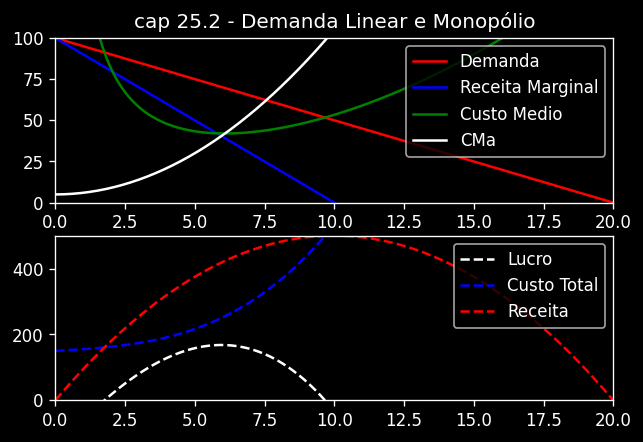
\includegraphics[scale=0.8]{cap25_2-demanda_linear_e_monopolio.png}
\end{center}

Para poder fazer essa simulação, eu tive de definir uma função custo e, consequentemente, uma função custo marginal\footnote{Eu tentei pensar numa função que apresentasse um comportamento parecido com a imagem que vemos no livro.}. Conseguimos ver que a curva de lucro tem um ponto de máximo exatamente onde a curva da receita marginal encontra o custo marginal. Qualquer ponto diferente desse levaria a um nível de lucro menor.
\\
\\
Além disso, também é relevante o fato da curva de custo médio estar abaixo da curva de demanda\footnote{Tente justificar isso matematicamente e, depois, tente criar uma situação onde isso acontece.}. Se o ponto de produção cuja receita marginal é igual ao custo marginal tiver um custo médio superior a demanda, a empresa receberá menos do que os custo de produção.\footnote{Veremos isso daqui a pouco no ponto 25.6.}.

\section{Estabelecimento de Preços com Markup}

Já conseguimos aprimorar nosso modelo de escolha da firma para o caso do monopolista. Agora que tornamos a receita marginal endógena, podemos ver as condições de maximização do lucro quando a firma tem poder de definir o preço ou a quantidade do mercado (mas não os dois ao mesmo tempo).
\\
\\
Podemos compreender essa última equação como uma política de preço do monopolista. Para isso, só precisamos isolar o termo $p(y)$ via rearranjo da última equação, o que após feito nos dá a seguinte relação

$$ p(y) = \frac{CMa(y)}{1 - 1/|\epsilon(y)|} $$
\\
Essa equação nos diz que o preço praticado no mercado cujo monopolista atua sempre\footnote{Sempre que ele agir de acordo com os pressupostos do nosso modelo de escolha.} se comportará como uma função de \textit{markup} do seu custo marginal. Podemos simplificar a visualização disso do seguinte modo

$$ p(y) = \phi \times CMa(y) $$
onde $\phi = \frac{1}{1 - 1/|\epsilon(y)|}$
\\
\\
Como sabemos, o monopolista sempre operará nos pontos cuja demanda é elástica\footnote{Ele até pode operar no ponto onde $\epsilon = 1$, já vimos que nesse caso, o resultado seria o mesmo do caso na competição perfeita.}, isso nos dará um $\epsilon(y) > 1$. Isso nos diz que o divisor $(1 - 1/|\epsilon|) <  1$, o que por sua vez, nos diz que $\phi > 1$.
\\
\\
Agora vamos dar uma olhada em um caso muito interessante: quando a curva de demanda possui a mesma elasticidade em todos os seus pontos.

\subsection{Demanda com Elasticidade Constante e Monopólio}

Para simular o caso da demanda com elasticidade constante, vamos usar o método do markup para encontrar o ponto de oferta do monopolista. Como esperado, teremos uma função de marcação acima da curva de custo marginal.

\begin{center}
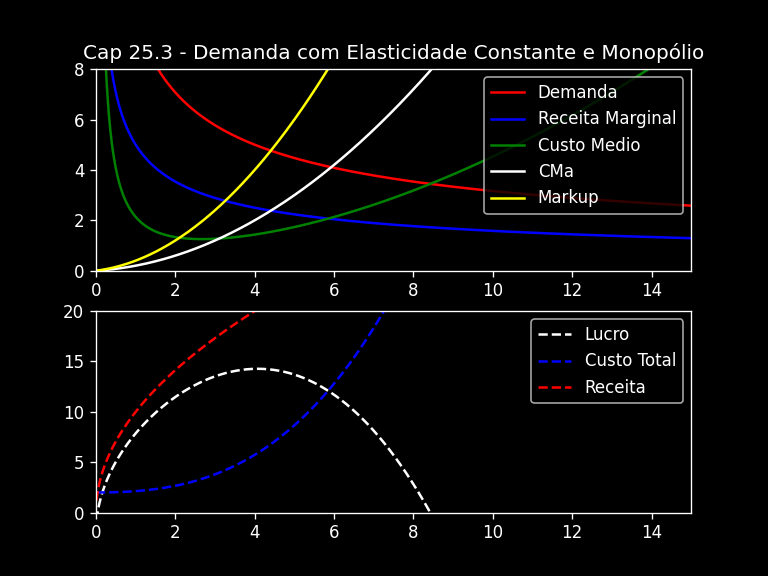
\includegraphics[scale=0.7]{cap25_3-demanda_ces_e_monopolio.png}
\end{center}

\textbf{Simulação:} \href{https://colab.research.google.com/drive/1MRJb9DZ7n_Hz2Kp9ng8K7pOcb1DTy_u5?usp=sharing}{Clique aqui} para ter acesso a essa simulação.
\\
\\
\textbf{Comentário:} Leia o exemplo sobre o impacto dos impostos sobre o monopolista na página 634. Com os conceitos vistos até agora, não deve ser difícil compreende-lo. Você pode acessar a simulação e modificar o custo variável para ver se o resultado é igual ao que você esperava.

\section{A Ineficiência do Monopólio}

Já conseguimos ver que, quando uma empresa opera como um monopólio, o preço de mercado será definido sempre acima do seu custo marginal. No mercado de competição perfeita, esse preço seria exatamente igual ao custo marginal. Isso implica na redução de algum excedente dos consumidores, mas em um incremento no excedente do produtor.
\\
\\
Como já sabemos, um arranjo é eficiente no sentido de Pareto se, e somente se, é possível realizar alguma troca de modo a se ter um aumento no excedente de uma das partes sem a redução do excedente de outra parte. Agora vamos investigar se o equilíbrio no mercado monopolista é eficiente. Considere a imagem abaixo.

\begin{center}
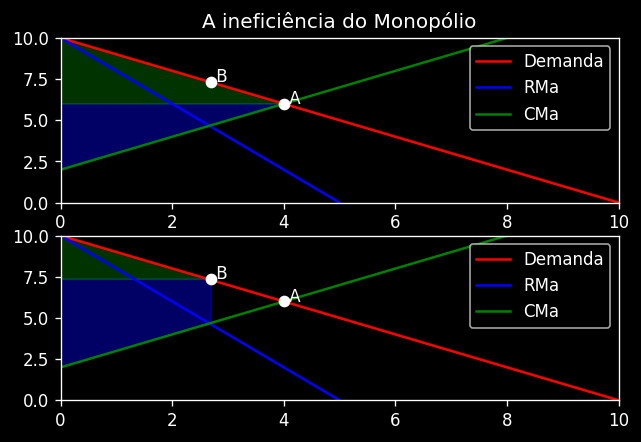
\includegraphics[scale=0.8]{cap25_4-inef_monopolio.png}
\end{center}

O gráfico da parte de cima é o equilíbrio no mercado de competição e o de baixo é o nosso equilíbrio com monopólio. Perceba como há um incremento no excedente do produtor (medido pela área azul) e uma redução do excedente do consumidor (área verde).
\\
\\
Para investigarmos se há uma ineficiência no sentido de Pareto no ponto $B$, façamos a seguinte pergunta: É possível adicionar uma unidade de produto no mercado de modo que o custo marginal pela produção desse bem seja inferior ao preço do mesmo? A resposta é claramente sim!
\\
\\
No nível $B$, a curva de preço (medida pela demanda inversa) ainda é superior à curva de custo marginal (aquela reta verde). Desse modo, se o monopolista produzisse mais uma unidade, ele receberia mais do que o custo marginal dessa unidade e os consumidores cujo preço de reserva é igual ao novo nível de preço passariam a consumir o produto. O excedente desse novo consumidor é igual a $0$, contudo, todos os que já consumiam o produto passaram a pagar menos do que antes o que aumentará os seus respectivos excedentes. Como o consumidor teria um lucro positivo (pois o custo marginal é inferior ao preço) e os consumidores teriam um aumento de excedente, achamos uma melhoria de Pareto.
\\
\\
A razão para o monopolista abrir mão dessa receita adicional é devida a necessidade dele de ter que manter o mesmo preço para todos os compradores\footnote{Vamos explorar mais essa ideia no próximo capítulo.}. Diferente da empresa na competição perfeita, ele leva em consideração o impacto dessa unidade adicional no lucro. Essa redução do lucro se dá porque ao produzir mais, o preço de todas as unidades cai. Se ele pudesse manter o preço nas unidades anteriores e vender mais barato as novas, ele venderia. 

\section{O Ônus do Monopólio}

Agora que já vimos que o monopólio é ineficiente, podemos querer mensurar o tamanho dessa ineficiência. Uma maneira possível de medir essa ineficiência é observando os excedentes nos cenários competitivo e de monopólio. Observe a figura abaixo:

\begin{center}
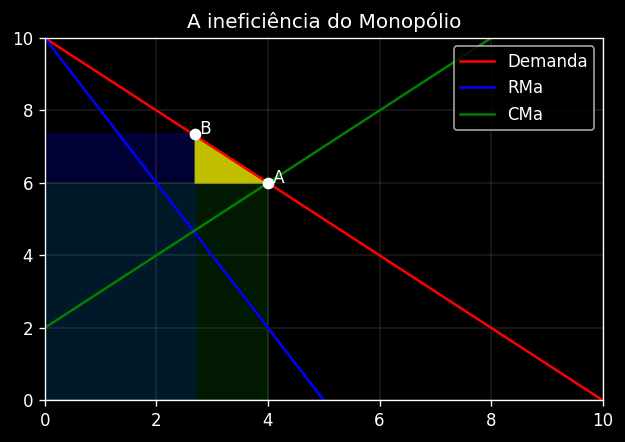
\includegraphics[scale=0.8]{cap25_5-onus_monopolio.png}
\end{center}

A área amarela é a medida da redução do excedente do consumidor. Em vermelho temos a redução do excedente do produtor. Em branco temos o quanto o monopolista consegue "capturar"\ do excedente dos consumidores ao adotar o nível de produção que maximiza o seu lucro.
\\
\\
A área branca não é definida como parte da ineficiência porque ela apenas demonstra uma transferência de excedente dos consumidores para o produtor. O \textbf{ônus resultante do monopólio} é precisamente a soma das áreas amarela e vermelha.
\\
\\
\textbf{Comentário:} Aqui o professor discorre sobre 3 exemplos do ônus do monopólio. Eu vou dar um resumo mas indico que você leia essa parte do livro.
\\
\\
No exemplo 1, vemos os casos das patentes (que, na prática, podem ser entendidas como um monopólio temporário). A ideia das patentes é criar um incentivo ao investimento em pesquisa e desenvolvimento de novas tecnologias. Contudo, por se tratar de um monopólio, acaba por criar um ônus atrelado a ele. O trabalho do Nobel William Nordhaus, demonstra que a estimativa da eficiência das patentes americanas é de 90\%, isso quer dizer que os consumidores estariam perdendo aproximadamente 10\% do seu excedente. O que parece indicar que o sistema de patentes não tem causado grandes malefícios.
\\
\\
No exemplo 2, ainda analisamos o mercado de patentes. Vemos que as patentes possuem 3 critérios de classificação: tempo de duração, extensão da proteção e novidade da invenção. Sendo os últimos dois muito subjetivos . Também discorremos sobre como o mercado de patentes permite algumas distorções (como o emaranhamento de patentes) de modo a tornar obrigatório para as empresas muito grandes a busca por grandes quantidades de patentes afim de se proteger de eventuais processos judiciais.
\\
\\
No exemplo 3, vemos o caso da isenção às proibições de \textit{antitrust} que os produtores agrícolas possuem nos EUA. Isso levou a uma pressão por parte dos grupos organizados dos produtores de batata a forçarem uma redução na quantidade ofertada do produto na ordem de 6,8 milhões de sacas. O que seria equivalente a 1,3 bilhão de pedidos de batata frita.

\section{Monopólio Natural}

Pois bem, já aprendemos o modelo de decisão do monopolista e também já vimos a ineficiência que esse modelo acarreta para os mercados. Ao percebemos que o monopólio produz aquém da quantidade ótima, poderíamos nos sentir tentados a propor regulações que obrigassem o monopolista a aumentar o seu nível de produção até o nível da competição perfeita. Contudo, esse problema é mais complexo do que parece, porque essa proposta de solução não leva em consideração a estrutura de custos.
\\
\\
Você mesmo pode fazer esse experimento, abra a simulação 25.2 ou a 25.3 e altere apenas o parâmetro "CF"\ que quer dizer "Custo Fixo". A medida que você aumenta esse parâmetro a curva de custo médio vai "subindo"\ e, em todos os pontos onde ele for superior a demanda, o monopolista terá lucro negativo.
\\
\\
Eu fiz 3 simulações para o caso da demanda com elasticidade constante. Uma com um custo fixo baixo, outra com um custo um pouco mais elevado e última com 10 vezes o custo fixo da primeira. Perceba ma imagem abaixo como a curva de lucro (da parte de baixo de cada painel vai caindo até desaparecer.

\begin{center}
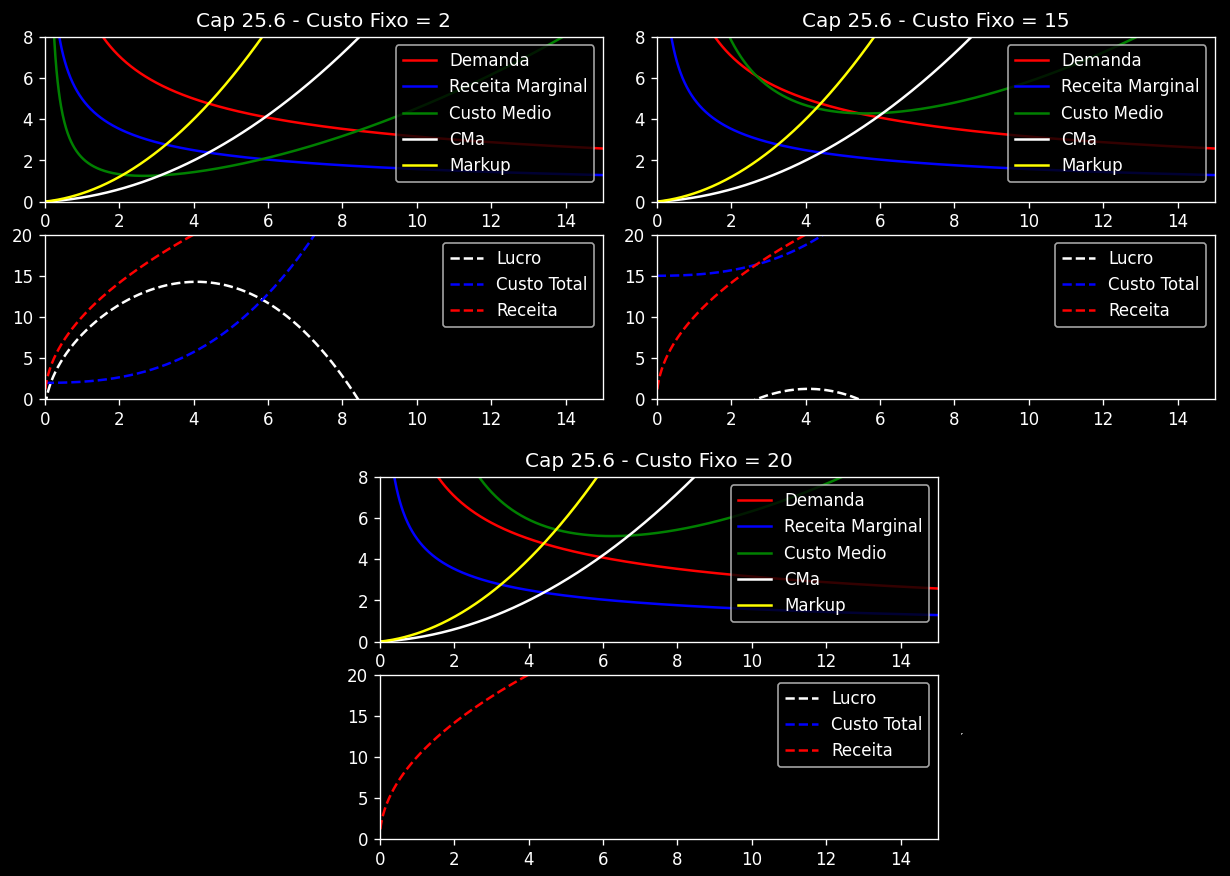
\includegraphics[scale=0.38]{cap25_6-monopolio_natural.png}
\end{center}

Chamamos de \textbf{monopólio natural} a situação onde temos uma estrutura de custo fixos fixos muito alta e custos marginais baixos. Agora podemos ver que se obrigarmos o monopolista a produzir o nível da competição perfeita, pode acontecer do projeto não ser sustentável, pois a curva de custo médio está acima da curva de demanda.
\\
\\
Agora o dilema ficou um pouco mais complexo. Se forçarmos o monopolista a produzir a quantidade que iguala o custo marginal ao preço, ele terá prejuízo. Se aceitarmos que ele mesmo defina a quantidade a produzir, agirá num ponto que produzirá uma ineficiência no mercado.
\\
\\
Não existe solução simples para essa questão. Na maioria das situações os monopólios naturais são regulamentados ou operados diretamente pelos governos. Cada opção de solução acaba acarretando benefícios e malefícios consigo. Em ambos os casos, os problemas são geralmente oriundos devido a informação assimétrica entre a empresa e os seus controladores.

\section{O Que Causa os Monopólios?}

Parabéns, querido aluno. Agora você já compreendeu como um monopolista age, o que o comportamento dele acarreta no mercado e como o controle sobre o monopólio é mais complexo do que se parece a primeira vista. Agora nos resta uma última investigação: Qual a causa dos monopólios?
\\
\\
Uma variável que podemos creditar como importante é a \textbf{escala mínima de eficiêntia (EME)}. Ela nada mais é do que o ponto de mínimo da nossa curva de custo médio.\footnote{Podemos achar esse ponto pela derivada primeira da função custo médio igual a zero e pela derivada segunda menor igual a zero.} O formato da curva de custo médio (e consequentemente a EME) é definido exclusivamente pela tecnologia.
\\
\\
Quando temos uma escala mínima de eficiência muito elevada, uma empresa precisa produzir uma quantidade muito grande dos bens vendidos no mercado para se manter. A economia é advinda da economia de escala. O que implica em uma capacidade produtiva de porte elevado. Nesses mercados, a chance maior é que hajam poucos ofertantes, e consequentemente, que esses ofertantes acabem usufruindo do poder de mercado advindo da pouca competitividade.
\\
\\
Quando temos uma EME pequena, qualquer empresa pequena pode começar a operar no mercado. Isso aumenta o número de competidores. O que acaba por reduzir o peso de cada empresa individualmente. O que acaba por gerar um ambiente de competição.
\\
\\
Observe que o fator importante é a relação entre a EME e o tamanho do mercado. É possível que a quantidade de eficiência aconteça em 10.000 de unidades, mas se o mercado for o Brasil inteiro, ainda pode ser que hajam muitos ofertantes. Quando não é possível aumentar o tamanho do mercado e a EME é elevada, aí sim, nos deparamos com uma condição de monopólio que pode necessitar de regulação ou mesmo intervenção do Estado.
\\
\\
Além da EME, outra maneira de se criar um monopólio é por meio da coordenação dos agentes ofertantes em uma \textbf{colusão}\footnote{Um ajuste secreto entre ofertantes para prejudicar outras pessoas.}. Quando um conjunto de empresa se une para definir em conjunto a produção, elas agem como um \textbf{cartel}. Esse cartel acaba atuando como se fosse um ofertante só (e consequentemente, age com o poder de mercado advindo dessa coordenação).
\\
\\
Um terceiro e último motivo para o nascimento de um monopólio é o bom e velho "cheguei primeiro". Se uma empresa, por algum acidente histórico, é a primeira a se estabelecer no mercado. É natural que ela se valha da falta de competidores e consiga um crescimento em escala. Quando novos ofertantes entram no mercado, o monopolista consegue usar seu arsenal de escala e reduzir artificialmente o preço até o ponto onde ninguém além dele pode se manter.
\\
\\
\textbf{Comentário:} Aqui o professor cita alguns exemplo. Mesma coisa de antes, indico ler o livro porque eu só vou dar uma resumida aqui.
\\
\\
No exemplo 1, vemos ocaso do mercado de diamantes e a sua gigante participante De Beers. É um exemplo de monopólio por tamanho da participação no mercado.
\\
\\
No exemplo 2, temos um caso de poder de mercado advindo da cooperação de comerciantes de móveis antigos.
\\
\\
No exemplo 3, outro exemplo de conluio por parte dos ofertantes para fixação dos preços de microchips de memória RAM.

%%%%%%%%%%%%%%%%%%%%%%%% CHAPTER %%%%%%%%%%%%%%%%%%%%%%%%
\chapter{O Comportamento do Monipolista}

\begin{chapquote}{The Godfather}
	``Great men are not born great, they grow great \dots''
\end{chapquote}

Na prática, a maioria das empresas possui algum poder de mercado. É bem possível que um mercadinho eleve um pouco seus preços sem que isso acarrete a perda de todos os seus clientes. Nesse capítulo vamos ver quais estratégias as empresas podem adotar para aumentar e explorar o seu poder de mercado.
\\
\\
A medida que você vai avançando no seu curso de Microeconomia, o seu arcabouço de conhecimento vai ficando cada vez mais refinado e, consequentemente, próximo da realidade. Os modelos puros de competição perfeita e monopólio até existem, mas são mais raros na realidade quando comparados à competição monopolística.\footnote{Veremos mais sobre isso nesse capítulo.}

\section{Tipos de discriminação de Preços}

No capítulo anterior, nós vimos que o monopolista acaba produzindo em um ponto onde a demanda ainda está disposta a pagar por mais do que o custo marginal. Vimos que a explicação do porquê ele não produz mais é que ele teria de baixar o preço de todos os produtos e não apenas os adicionais. Pois bem, existem alguns monopolistas que detém o poder de \textbf{discriminação de preços}. O professor classifica esse poder em 3 categorias:

\begin{itemize}
\item Discriminação de Preços de 1º Grau:
	\begin{itemize}
	\item[] Nesse caso ele tem poder de cobrar um preço diferente para cada consumidor e para cada quantidade.
	\end{itemize}
\item Discriminação de Preços de 2º Grau
	\begin{itemize}
	\item[] Nesse caso ele tem poder de discriminar o preço apenas para as quantidades compradas. Mas todos os consumidores que levarem a mesma quantidade, pagarão o mesmo preço no total.
	\end{itemize}
\item Discriminação de Preços de 3º Grau
	\begin{itemize}
	\item[] Esse é o caso mais comum. É quando o monopolista tem o poder de escolher qual preço cada pessoa vai pagar por todas as unidades que levar. Ou seja, ele pode controlar qual o valor de todas as unidades da cesta, contudo, não pode diferenciar o valor entre essas unidades.
	\end{itemize}
\end{itemize}

\section{Discriminação de Preços de 1º Grau}

Nesse caso, o monopolista está em \href{https://www.encurtador.com.br/eqCN1}{plenos poderes}. Ele possui conhecimento do preço de reserva\footnote{Lembra desse conceito?} de cada consumidor e, com esse conhecimento, cobra exatamente o valor máximo para cada quantidade. Também chamamos esse tipo de \textbf{discriminação perfeita}.
\\
\\
Um fato curioso desse arranjo é que, por incrível que pareça, ele é eficiente no sentido de Pareto. Uma vez que, para cada produto vendido, os consumidores pagam exatamente o valor máximo que estão dispostos a pagar, e consequentemente, o monopolista vai vender para todos os consumidores que tenham um preço de reserva maior ou igual ao custo marginal. O ponto final da produção será o ponto onde a quantidade iguala o custo marginal à curva de demanda.
\\
\\
Em termos de excedente, o que acontece é que o monopolista captura todo o excedente do mercado. Os consumidores, por sua vez, não possuem nenhum excedente.

\begin{figure}[H]
\centering
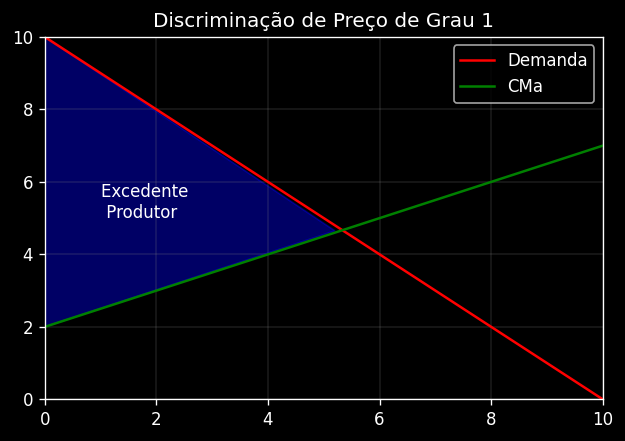
\includegraphics[scale=0.6]{cap26_2-discriminacao_grau1.png}
\end{figure}

Uma maneira conveniente se se pensar nessa situação é pela ótica da produção. Ao invés de pensar que o produtor olha para cada cliente e consegue cobrar exatamente o máximo que ele quer pagar, ele simplesmente oferta no mercado uma quantidade e deixa que os clientes definam quanto pagarão por ela. Claro que estamos supondo uma simplificação do comportamento das pessoas, mas a ilustração é válida.
\\
\\
O professor cita um exemplo da companhia aérea chamada Southwest Airlines. Que usou um software chamado Ding que faz ofertas periódicas e exclusivas para cada cliente cadastrado no sistema. Outro exemplo menos real, e mais icônico, é Mafioso Don Vito Corleone da clássica trilogia de filmes The Godfather (na abertura de todos os capítulos desse manual contém uma frase retirada dessa obra). O "modelo de negócio"\ do protagonista é fazer alguns favores em troca de outros favores. No caso do personagem mafioso, ele abusava do poder de mercado que detinha para cobrar o máximo possível (em bens ou serviços) de quem estava em dívida com ele.
\\
\ 
\\
\begin{figure}[H]
\centering
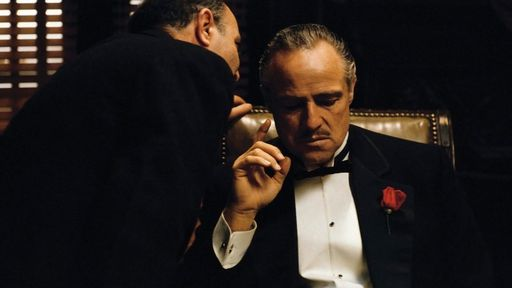
\includegraphics[scale=0.5]{cap26_2-don_corleone.jpeg}
\caption*{The Godfather (1972) - Paramount Films}
\end{figure}

\section{Discriminação de Preços de 2º Grau}

Nesse modelo, também chamado de \textbf{fixação de preços não linear}, o produtor já não pode cobrar, por uma mesma quantidade, um valor diferente entre consumidores diferentes. Isso força o monopolista a desenvolver uma estratégia de precificação que tente tirar o maior proveito possível das diferentes curvas de demanda.
\\
\\
\textbf{Comentário:} Eu não sei você, mas no meu caso, deu um trabalhão para entender o que o professor quis dizer nessa parte. Eu acho que o que deixou mais confuso foi ele ter suposto que o custo marginal é igual a zero (porque isso implicaria em dizer que ele venderia alguma cesta ao preço zero). Então eu retirei essa simplificação e reconstruí a mesma argumentação dele só que para um custo marginal constante maior que zero.\footnote{\href{https://www.youtube.com/watch?v=OBgziVdHH8w}{Esse vídeo aqui me ajudou bastante a entender melhor o que o professor quis dizer.}}
\\
\\
Imagine que temos apenas $2$ grupos de consumidores no mercado. Como nosso modelo prevê, o monopolista tem acesso as curvas de demanda de cada consumidor, mas como limitação, ele só pode escolher quais cestas ofertar por qual preço, e deixar que os consumidores escolham qual é a melhor para eles. Chamamos esse modelo de \textbf{autosseleção}.
\\
\\
O objetivo do monopolista é captar todo o excedente do mercado. Mas ele enfrenta uma limitação nessa modalidade de discriminação de preços. Como ele não pode vender a mesma quantidade a preços diferentes para os grupos de consumidores, ele tem de escolher se vai vender a preço de reserva da curva de demanda 1 ou 2.

\begin{figure}[H]
\centering
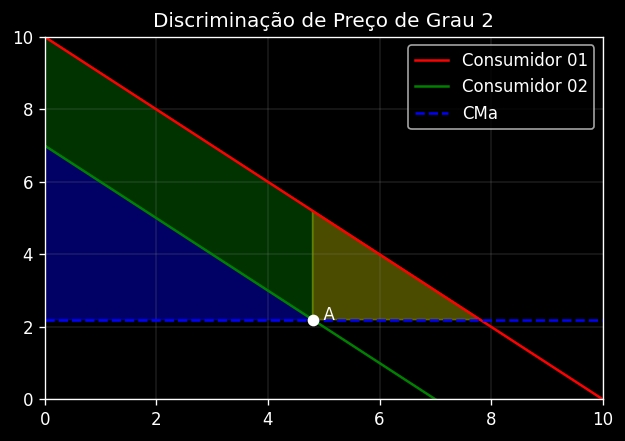
\includegraphics[scale=0.8]{cap26_3-discriminacao_grau2_1.png}
\end{figure}

Se ele optar por vender na fronteira da curva de demanda 1, ele vai abrir mão de todo o excedente advindo dos consumidores do tipo 2! Isso significaria abrir mão do toda a área azul na figura acima. Como ele não vai fazer isso, ele adotará a seguinte abordagem: Vender de $0$ até o ponto $A$ pelo preço de reserva da curva de demanda dos consumidores do tipo 2 e, a partir desse ponto, vender pela fronteira do preço de reserva dos consumidores do tipo 1. Isso garantirá que ele obtenha todo o excedente da área azul e também da área amarela.
\\
\\
Não satisfeito, o monopolista pode pensar um pouco mais e perceber que ele pode escolher uma opção que aumentará o seu excedente. Veja o que acontece se ele decide optar pela fronteira do consumidor tipo para uma cesta cuja quantidade é um pouco menor que a cesta $A$.

\begin{figure}[H]
\centering
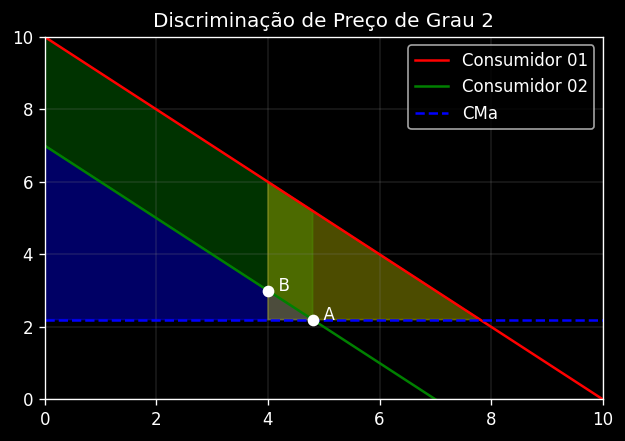
\includegraphics[scale=0.8]{cap26_3-discriminacao_grau2_2.png}
\end{figure}

Veja só que interessante, como no ponto $B$ o preço não é igual ao custo marginal para o consumidor tipo 2, haverá uma perda no total do excedente capturado pelo monopolista, mas em contrapartida, veja como a área amarela aumentou muito mais do que a área de perda do excedente do primeiro grupo. Isso quer dizer que, ao aumentar o preço da cesta, optando por adotar o preço de reserva do consumidor tipo 1 em um ponto anterior ao custo marginal igual à demanda tipo 2, o monopolista "abre mão"\ de uma pequena parte do excedente tipo 1 e ganha uma grande parte do excedente tipo 2. Não é difícil prever que ele continuará reduzindo a quantidade até o ponto onde o excedente perdido de um grupo é igual ao excedente ganho do outro.

\begin{figure}[H]
\centering
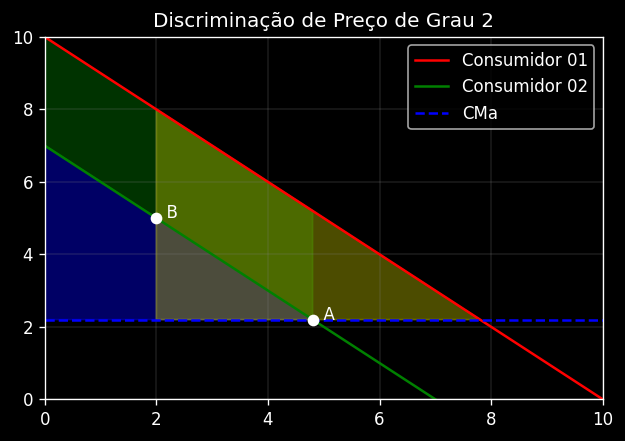
\includegraphics[scale=0.8]{cap26_3-discriminacao_grau2_3.png}
\end{figure}

A partir desse novo ponto $B$, o excedente perdido dos consumidores tipo 2 com o aumento do preço da cesta é maior que o ganho adicional do excedente dos consumidores tipo 1. Desse modo o monopolista acaba com um excedente total igual à área azul e toda a área amarela.
\\
\\
\textbf{Comentário:} Alguns de vocês podem pensar que o excedente abaixo da curva de demanda verde foi inteiramente perdido. Mas não é o caso! Perceba que, mesmo com a retirada dos consumidores do tipo $2$, essa área de excedente foi preenchida pelo excedente dos consumidores do tipo $1$. O monopolista abre mão no sentido que antes essa área era computada duas vezes (uma vez para cada tipo de consumidor).
\\
\\
Na realidade, o principal método de incentivo a autosseleção é a alteração da qualidade do bem. Normalmente, o monopolista reduz a qualidade dos produtos direcionados aos consumidores com preços de reserva menores, afim de eviter que seus consumidores dispostos a pagar mais, prefiram comprar esses produtos ao invés de produtos de "primeira linha". Essa estratégia maximiza o lucro do monopolista e ainda garante algum excedente para os consumidores das demandas mais altas.
\\
\\
O professor coloca dois exemplos que são espetaculares. Um sobre a diferença nos preços das passagens aéreas e o motivo da existência das classes econômica e executiva nos meios de transporte. Recomendo demais a leitura. O segundo é referente ao mercado de remédios.

\section{Discriminação de Preços de 3º Grau}

Só nos resta o último tipo de discriminação de preços. Nesse caso, o monopolista consegue discernir claramente qual consumidor pertence a qual grupo e, consequentemente, consegue cobrar um preço diferente. Atente para o fato que o monopolista só pode adota um único preço para cada grupo de consumidores.
\\
\\
Na prática, a modelagem desse problema é muito parecida com o que vimos no capítulo passado, já que, ele só pode escolher um único preço para cada tipo de consumidor. A única diferença do modelo do capítulo passado é que ele vai se deparar com mais de uma curva de demanda. Veja a formalização do problema logo abaixo

\begin{center}
\LARGE $\stackrel{máx}{\text{\small $y_1,y_2$}} \ \ \stackrel{p_1(y_1)y_1 + p_2(y_2)y_2 - c(y_1 + y_2)}{\ }$ \\
\end{center}

Esse problema nada mais é do que uma adaptação do problema da maximização da receita. Veja que $p_1(y_1)y_1$ nada mais é do que a receita obtida com a venda do produto para o grupo 1. Desse modo, o problema de maximização é a receita total obtida (que é a soma das receitas da venda para cada grupo) menos o custo total de produção.
\\
\\
Da mesma maneira de antes, a otimização será dada por:

$$ RM_1(y_1) = CMa(y_1+y_2) $$
$$ RM_2(y_2) = CMa(y_1+y_2) $$
Isso claramente implica em
$$ RM_1(y_1) = RM_2(y_2) = CMa(y_1+y_2) $$

\textbf{Atenção:} Eu acho que encontrei um erro de tradução no parágrafo que vem logo depois dessa expressão das receitas marginais acima. Na tradução, temos o trecho: "se a receita marginal no mercado 1 ultrapassar o custo marginal, valeria a pena aumentar a produção \textbf{nos dois mercados}". Isso está errado! No original temos a seguinte passagem: "if the marginal revenue in market 1 exceeded marginal cost, it would pay to expand output \textbf{in market 1}, and similarly for market 2". Uma tradução melhor seria algo como: "se a receita marginal no mercado 1 for maior que a o custo marginal, então valerá a pena aumentar a produção no mercado 1, a mesma lógica se aplica ao mercado 2".
\\
\\
Podemos usar a nossa fórmula da elasticidade para elaborar um pouco mais esse problema:

$$ p_1(y_1) \left[1 - \frac{1}{|\epsilon_1(y_1)|} \right] = CMa(y_1 + y_2) $$
$$ p_2(y_2) \left[1 - \frac{1}{|\epsilon_2(y_2)|} \right] = CMa(y_1 + y_2) $$
\\
Suponha que $y_1 = y_2$. Se $p_1 > p_2$, então:

$$ 1 - \frac{1}{|\epsilon_1(y_1)|} < 1 - \frac{1}{|\epsilon_2(y_2)|} $$
\\
O que implica em

$$ \frac{1}{|\epsilon_1(y_1)|} > \frac{1}{|\epsilon_2(y_2)|} $$
\\
Que, por fim, nos diz que

$$ |\epsilon_1(y_1)| < |\epsilon_2(y_2)| $$
\\
Não continue lendo se você não entendeu essa afirmação. Pare e pense até sentir que compreendeu o argumento. Se ainda tiver dúvida \href{https://twitter.com/bruno_ruas2}{me manda um twite que eu te ajudo}.
\\
\\
Dessa maneira, podemos ver que quanto mais elástico for o mercado, menor será o seu preço. Faz todo sentido porquê quanto mais elástica é a demanda, mais sensível ela será às alterações de preços. Portanto, o monopolista vai conseguir elevar o preço sempre que a demanda for inelástica e manterá o preço comparativamente mais baixo nos grupos de demanda mais elástica. Isso maximizará o seu lucro em cada grupo de consumidores.
\\
\\
\textbf{Comentário:} Querido aluno, agora você tem todo o arcabouço teórico necessário para entender o motivo de você pagar meia entrada no cinema\footnote{Entender isso é muito top, fala sério.}. Os cinemas acreditam que uma elevação dos preços levaria vocês a buscar outros serviços além do cinema, visto que é comum supor que essa fase da vida tenha restrição orçamentária consideravelmente modesta. Por outro lado, um executivo de uma empresa tem um preço de reserva muito maior que o de vocês, então o cinema cobra dele mais caro para entrar (sem falar o preço "salgado"\ das pipocas).
\\
\\
Agora o professor coloca três exemplos. O primeiro é teórico, o segundo é um exemplo de aplicação e o terceiro é uma aplicação do conceito ao mercado de revistas acadêmicas. Eu vou criar uma simulação do segundo exemplo.

\subsection{Curvas de Demanda Lineares}

O monopolista precisa lidar com duas curvas de demanda (que suporemos serem lineares) do tipo:

$$ D_1(p_1) = 100 - p_1 $$
$$ D_2(p_2) = 100 - 2p_2 $$
\\
As demandas inversas dessas funções são

$$ p_1(y_1) = 100 - y_1 $$
$$ p_2(y_2) = 50 - y_2/2 $$
\\
As funções de receita serão iguais a

$$ r_1(y_1) = 100y_1 - y_{1}^{2} $$
$$ r_2(y_2) = 50y_2 - \frac{y_{2}^{2}}{2} $$
\\
Cujas receitas marginais serão

$$ RMa_1(y_1) = 100 - 2y_{1} $$
$$ RMa_2(y_2) = 50 - y_{2} $$
\\
Para simplificar vamos supor que o custo marginal é contante em $CMa = \$ 20,00 $. Com isso já podemos criar uma simulação do modelo. Mas antes de colocar o computador fazer isso, nós podemos encontrar os pontos de máximo facilmente ao igualar as funções de receita marginal ao custo marginal.

$$ 100 - 2y_{1} = 20 \hspace{100pt} 50 - y_{2} = 20 $$
$$ 100 - 20 = 2y_{1} \hspace{100pt} 50 - 20 = y_{2} $$
$$ 80/2 = y_{1} = 40 \hspace{120pt} y_2 = 30 $$
\\
Sabemos que os pontos de maximização do lucro para cada curva de demanda serão os pontos cujas quantidades são iguais a $y_1 = 40$ e $y_2 = 30$. Para descobrir os preços, basta colocar esses valores nas funções de demanda inversa. Podemos ver que esses são os pontos que estão no topo das curvas de lucro 1 e 2.

\begin{figure}[H]
\centering
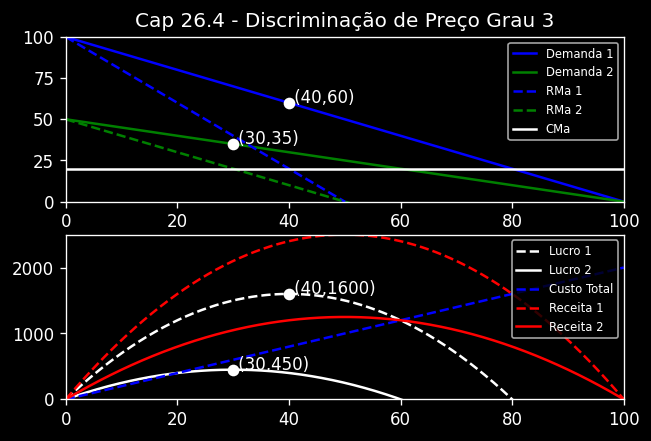
\includegraphics[scale=0.8]{cap26_4-discriminacao_grau3.png}
\end{figure}

\textbf{Simulação:} \href{https://colab.research.google.com/drive/1TYSpJLSEg4yInKX_viA6aP8qLiRsHdBm?usp=sharing}{Clique aqui} para ter acesso a essa simulação.
\\
\\
Se, por outro lado, o monopolista não puder fazer essa separação dos preços, teremos que somar as demandas como se fosse uma única e trabalhar a otimização como no primeiro modelo do capítulo 25.

\begin{figure}[H]
\centering
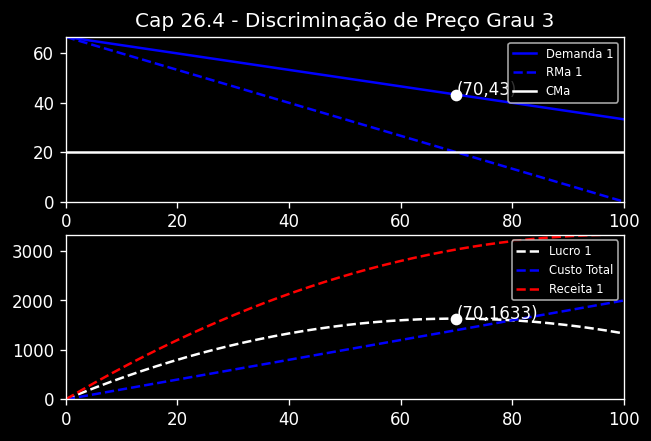
\includegraphics[scale=0.8]{cap26_4-discriminacao_grau3_2.png}
\end{figure}

\textbf{Atenção: } Quando trabalharmos com demandas somadas, temos que testar se o preço de equilíbrio não gera demanda negativa em alguma das curvas de demanda. Se a função demanda for negativa ao preço de equilíbrio, isso quer dizer que o monopolista aumentará o seu lucro se não vender para esse grupo de consumidores. Ao excluir essa demanda e calcular o novo equilíbrio, seu lucro aumentará.

\section{Vinculação de Produtos}

Uma prática muito comum entre as empresas é a \textbf{venda casada}. Você já se perguntou qual o motivo das empresas de internet se esforçarem tanto para vender o pacote TV + Internet + Telefone?. Pois bem, agora você vai ter uma ideia por trás dessa estratégia.\footnote{Aqui estamos supondo que as demandas por esses serviços não são relacionadas. Mas não leve esse primeiro parágrafo tão ao pé da letra. O objetivo dele é só vender o conteúdo do tópico ;)}
\\
\\
Já vimos que a vontade do monopolista é cobrar o máximo possível para cada cliente em cada quantidade. Isso faria com que ele capturasse todo o excedente do mercado. Como na prática isso implicaria em conhecimento perfeito de todos os consumidores e existe uma legislação que limita a capacidade de impor muito do poder de mercado, as empresas se valem de estratégias para maximizar esse excedente.
\\
\\
Uma dessas estratégias é exatamente a venda casada. A ideia é a seguinte: como o vendedor não pode cobrar um preço para cada consumidor, ele precisa ter uma ideia dos preços de reserva dos mesmos para que possa cobrar exatamente o valor do preço de reserva mais baixo que o custo marginal permita.
\\
\\
Veja a tabela 26.1 a página 672 do livro. Temos dois tipos consumidores que possuem preços de reservas inversos para dois tipos de programas diferentes. Se o monopolista cobrar $U\$ 101,00$ pelo processador de texto, ele perderá 100\% dos consumidores do tipo A. Por causa disso, ele sempre cobrará o mínimo possível para poder capturar o preço de reserva mais baixo. Isso implica que os consumidores que possuem preços de reserva maiores tenham algum excedente.
\\
\\
Mas como bem sabemos, as empresas sempre pensam em novas estratégias. No caso da vinculação de produtos, supondo que o preço de reserva pelos produtos juntos seja igual à soma dos preços individuais, nós tratamos os dois produtos como uma cesta única. Nesse novo arranjo, o vendedor consegue cobrar um preço maior, porque o preço de reserva por cesta é maior que o valor cobrado separadamente.
\\
\\
Eu expandi um pouco do exemplo do professor Varian para um caso de 1.000 consumidores. Nessa simulação os preços de reserva são aleatórios entre 51 e 100. Depois eu testei as duas abordagens e comparei os lucros a medida que se eleva o preço praticado no mercado. Para efeito de simplificação, os preços de reserva mínimos são iguais nos dois produtos, então o vendedor sempre aumentará os preços em paralelo. Atente para o fato de que nesse gráfico o preço está no eixo horizontal.\footnote{Ficou na dúvida, fala comigo que eu explico melhor.}

\begin{figure}[H]
\centering
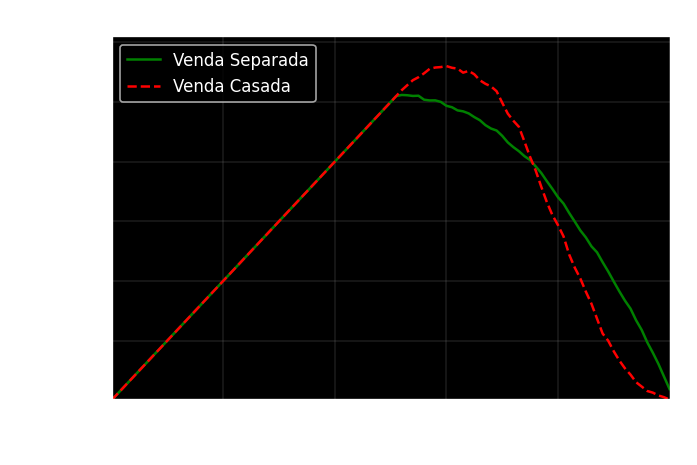
\includegraphics[scale=0.8]{cap26_5-venda_casada.png}
\end{figure}

\textbf{Simulação:} \href{https://drive.google.com/file/d/1WhxGaAhUB9dKkgrKWadihIrzS4cm3bXP/view?usp=sharing}{Clique aqui} para ter acesso a essa simulação.
\\
\\
De zero até 50, a curva de lucro é uma linha reta porque o preço de reserva mínimo da nossa simulação é 50. Então, sempre existirá alguém disposto a comprar a medida que ofertamos até esse preço. A partir desse ponto, cobrar mais caro implica em abrir mão dos consumidores com preço de reserva menor que o preço.

\section{Tarifas Bipartidas}

Um artigo famoso de 1971 cujo título é "A Disneyland Dilemma: Two-Part Tariffs for a Mickey Mouse Monopoly", de Walter Oi, nos mostra uma situação interessante. Como o monopolista se comportará no caso da venda de dois produtos que possuem demandas interrelaciandas?
\\
\\
No tópico anterior, supomos que as demandas eram independentes. Agora temos um caso onde, ao aumentar a oferta do bem 1, os consumidores estarão menos propensos a consumir o bem 2. Chamamos esse arranjo de \textbf{tarifa bipartida}.
\\
\\
Como já trabalhamos antes, sabemos que a maximização do lucro é obtida no ponto onde o custo marginal é igual à receita marginal. Fazendo isso para a oferta do bem 1 e como ele não pode discriminar perfeitamente os preços, haverá um excedente do consumidor. Esse excedente é exatamente o valor máximo que ele pode cobrar pelo bem 2. Nesse caso, pode ser que a quantidade cobrada pelo bem 2 seja inferior ao montante que iguale o custo marginal à receita marginal.
\\
\\
Para elucidar esse modelo eu fiz uma simulação. Fora suposto que as demandas são lineares, com a mesma forma funcional e interdependentes, ou seja, quanto mais de um bem se tem, menos do outro terá. Os custo marginais são fixos em 20.
\\
\\
Como esse problema envolve o equilíbrio em dois mercados (bem 1 e bem 2), eu optei por construir um gráfico tridimensional. O problema dessa abordagem é que a melhor maneira de se entender um gráfico desse é pela mudança do ângulo da câmera. Então eu vou colocar 3 perfis de visualização mas também fiz um gif com um panorama dos eixos \href{https://github.com/brunoruas2/Meus_Estudos/blob/main/Microeconomia/Microeconomics\%20-\%20Hal\%20Varian/images/cap26_6-tarifas_bipartidas.gif}{\textbf{clique aqui para ver}}.

\begin{figure}[H]
\centering
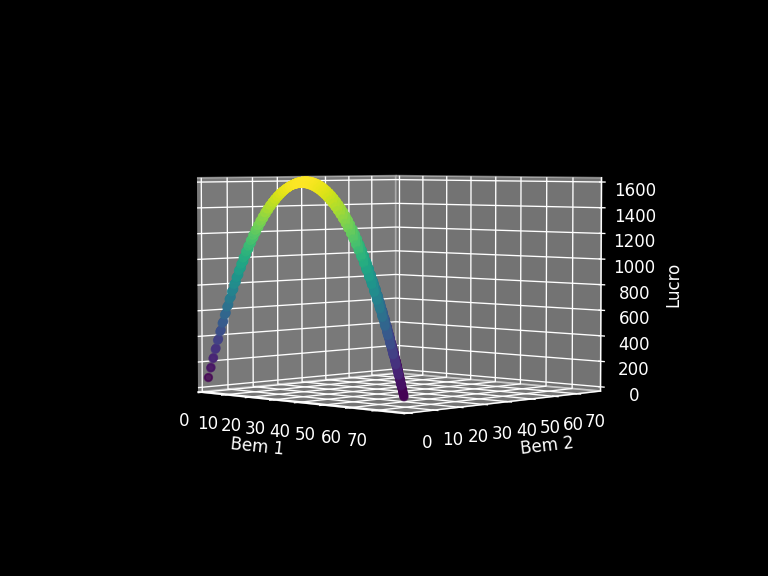
\includegraphics[scale=0.6]{cap26_6-tarifas_bipartidas1.png}
\end{figure}

Nessa primeira imagem temo um ângulo que evidencia como o lucro se comportaria se só existisse o mercado do bem 1. Podemos ver que o lucro é maximizado em um ponto (que é justamente onde o custo marginal é igual à receita marginal. A segunda imagem é similar a primeira, mas para o outro bem.

\begin{figure}[H]
\centering
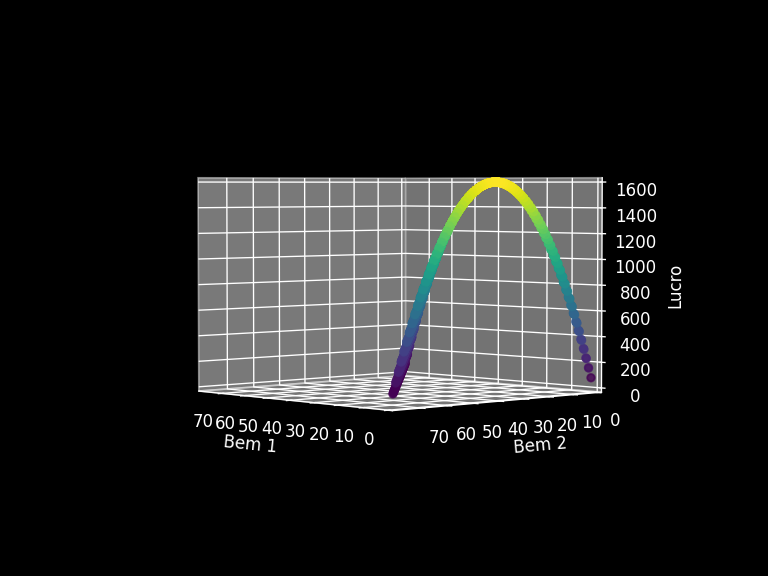
\includegraphics[scale=0.6]{cap26_6-tarifas_bipartidas2.png}
\end{figure}

A terceira mostra como o monopolista deverá agir para poder ofertar ambos os bens. O padrão é simétrico porque no modelo as duas demandas possuem as mesmas formas e os mesmos coeficientes. Veja como a figura do lucro forma um tipo de "onda"\ que parte da cesta onde os dois bens são iguais a zero. Na parte amarela temos o máximo do lucro possível para cada cesta. E, a partir desses pontos de máximo, os lucros de cada cesta vão sendo cada vez menores.

\begin{figure}[H]
\centering
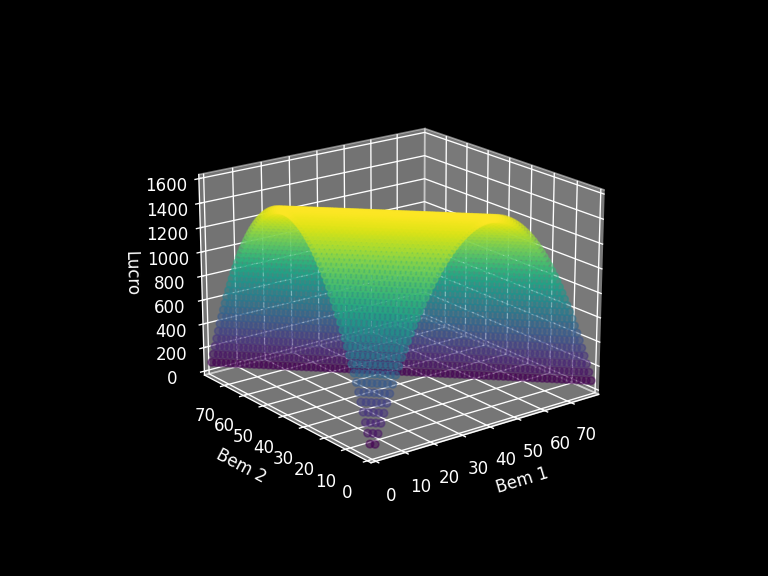
\includegraphics[scale=0.8]{cap26_6-tarifas_bipartidas3.png}
\end{figure}

A última mostra um ângulo onde vemos a relação de troca entre os bens (a linha vermelha indica a reta onde as cestas maximizam o lucro). Veja que, visto de cima, temos um gráfico que demonstra o quanto o monopolista tem que abrir mão de um bem para vender mais do outro, sem que isso incorra em redução do seu lucro total.

\begin{figure}[H]
\centering
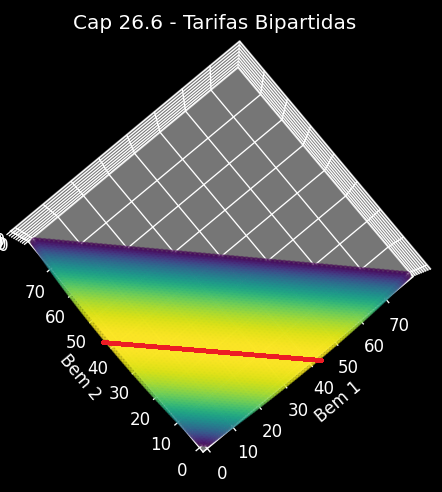
\includegraphics[scale=0.60]{cap26_6-tarifas_bipartidas4.png}
\end{figure}

Como as demandas desse modelo são simétricas, o modelo gráfico é uniforme. Na imagem abaixo eu simulei o mesmo modelo para o caso onde o custo marginal do bem 2 é igual a zero.

\begin{figure}[H]
\centering
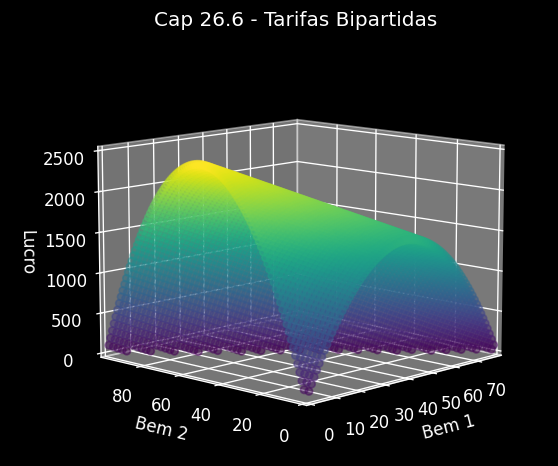
\includegraphics[scale=0.75]{cap26_6-tarifas_bipartidas5.png}
\end{figure}

Podemos ver claramente que, nesse segundo caso, o monopolista só maximiza seu lucro ao vender exclusivamente o bem 2.
\\
\\
Essa assimetria é a explicação do motivo da Disney não cobrar um preço pela entrada nos brinquedos. Existe uma assimetria em os custos dos serviços. A Disney percebeu que ao cobrar somente a entrada, poderia captar mais o excedente total do mercado do que se cobrasse também os passeios aos brinquedos.

\section{Competição Monopolística}
\section{Modelo de Diferenciação de Produtos por Local}
\section{Diferenciação de Produtos}
\section{Mais Sorveteiros}

%%%%%%%%%%%%%%%%%%%%%%%% CHAPTER %%%%%%%%%%%%%%%%%%%%%%%%
\chapter{O Mercado de Fatores}

%%%%%%%%%%%%%%%%%%%%%%%% CHAPTER %%%%%%%%%%%%%%%%%%%%%%%%
\chapter{O Oligopólio}

%%%%%%%%%%%%%%%%%%%%%%%% CHAPTER %%%%%%%%%%%%%%%%%%%%%%%%
\chapter{A Teoria dos Jogos}

%%%%%%%%%%%%%%%%%%%%%%%% CHAPTER %%%%%%%%%%%%%%%%%%%%%%%%
\chapter{Aplicações da Teoria dos Jogos}

%%%%%%%%%%%%%%%%%%%%%%%% PART %%%%%%%%%%%%%%%%%%%%%%%%
\part{Tópicos Avançados}

%%%%%%%%%%%%%%%%%%%%%%%% CHAPTER %%%%%%%%%%%%%%%%%%%%%%%%
\chapter{Economia Comportamental}

%%%%%%%%%%%%%%%%%%%%%%%% CHAPTER %%%%%%%%%%%%%%%%%%%%%%%%
\chapter{Trocas}

%%%%%%%%%%%%%%%%%%%%%%%% CHAPTER %%%%%%%%%%%%%%%%%%%%%%%%
\chapter{Produção}

%%%%%%%%%%%%%%%%%%%%%%%% CHAPTER %%%%%%%%%%%%%%%%%%%%%%%%
\chapter{O Bem-Estar}

%%%%%%%%%%%%%%%%%%%%%%%% CHAPTER %%%%%%%%%%%%%%%%%%%%%%%%
\chapter{Externalidades}

%%%%%%%%%%%%%%%%%%%%%%%% CHAPTER %%%%%%%%%%%%%%%%%%%%%%%%
\chapter{Tecnologia da Informação}

%%%%%%%%%%%%%%%%%%%%%%%% CHAPTER %%%%%%%%%%%%%%%%%%%%%%%%
\chapter{Bens Públicos}

%%%%%%%%%%%%%%%%%%%%%%%% CHAPTER %%%%%%%%%%%%%%%%%%%%%%%%
\chapter{Informação Assimétrica}

\end{document}
